\chapter{Sequenzdiagramm}

\begin{tiny}
PC
\end{tiny}

Als Beispiel für den Datenfluss im System \grqq ofCourse\grqq\ soll das nachfolgende Sequenzdiagramm dienen. Dabei wird der Verlauf einer Kursanmeldung mit auftretendem Fehler beschrieben.

\section{Fallbeschreibung}

Nach erfolgreicher Anmeldung befindet sich der Nutzer aktuell auf der Seite \grqq search.xhtml\grqq\ um nach einem angebotenen Kurs zu suchen mit dem Vorhaben, sich für diesen zu registrieren. Zuerst wird der gewünschte Suchbegriff vom Nutzer eingegeben. Anschließend wird die Anfrage bearbeitet und eine Liste mit Ergebnissen auf der gleichen Seite angezeigt. Der Nutzer klickt auf einen Kurs zu dem er sich anmelden möchte und wird auf die entsprechende Seite \grqq courseDetails.xhtml\grqq\ mit den Kursdetails weitergeleitet. Hier möchte sich der Nutzer anmelden und klickt auf den entsprechenden Button. Die Aktion kann allerdings nicht durchgeführt werden wegen eines systeminternen Abbruchs der Verbindung zur Datenbank. Daraufhin erscheint eine Fehlermeldung, der Nutzer bleibt auf der Seite zu den Kursdetails.

\section{Diagramm}

Nachfolgend das Sequenzdiagramm zum beschriebenen Fall. Dazu noch einige Anmerkungen:

\begin{itemize}

\item Die blauen, gestrichelten Linien unmittelbar nach dem dritten HTTP-request des Clients dienen als Platzhalter. An dieser Stelle im Diagramm wiederholt sich der gesamte Datenfluss zwischen dem zweiten HTTP-request des Clients und dem zweiten HTTP-response. Einzige Ausnahme in diesem Block bilden die X, welche eine Objektzerstörung darstellen. Hier werden die Lebenslinien nach unten hin länger gezogen. Die Objekte \texttt{model.Course} und \texttt{model.CourseUnit} werden auf einer Ebene wie \texttt{action.CourseDetailBean} zerstört.

\item Methodenaufrufe innerhalb der \texttt{create} Sequenzen werden der Übersichtlichkeit halber im Diagramm ausgelassen. Nachfolgend eine Auflistung dieser Methoden:

	\begin{itemize}
	\item \texttt{model.Course}:
		\begin{itemize}
		\item \texttt{setCourseID(courseID:int)}
		\item \texttt{setTitle(title:String)}
		\item \texttt{setNextCourseUnit(nextCourseUnit:CourseUnit)}
		\item \texttt{setStartDate(startDate:Date)}
		\item \texttt{setEndDate(endDate:Date)}
		\item \texttt{setMaxUsers(maxUsers:int)}
		\item \texttt{setCourseImage(image:String)}
		\item \texttt{setDescription(description:String)}
		\item \texttt{setCourseUnits( courseUnits:List<CourseUnit>)}
		\item \texttt{setCourseAdmins( coursAdmins:List<User>)}
		\item \texttt{setUsers(users:List<User>)}
		\item \texttt{setUsersToInform( usersToInform:List<User>)}
		\end{itemize}
	\end{itemize}
	
	\begin{itemize}
	\item \texttt{model.CourseUnit}:
		\begin{itemize}
		\item \texttt{setCourseUnitID(courseUnitID:int)}
		\item \texttt{setTitle(title:String)}
		\item \texttt{setDescription(discription:String)}
		\item \texttt{setStarttime(startingTime:Date)}
		\item \texttt{setEndtime(endTime:Date)}
		\item \texttt{setAddress(address:Address)}
		\item \texttt{setPrice(price:float)}
		\item \texttt{setMaxUsers(maxUsers:int)}
		\item \texttt{setMinUsers(minUsers:int)}
		\item \texttt{setCourseAdmins( courseAdmin:List<User>)}
		\item \texttt{setUsers(users:List<User>)}
		\item \texttt{setCourseImage(image:String)}
		\item \texttt{setLocation(location:String)}
		\end{itemize}
	\end{itemize}
	
\item Innerhalb der oben erwähnten \texttt{create} Sequenzen werden Objekte der DTOs \texttt{model.User} und \texttt{model.Address} erstellt, welche ebenfalls der Übersichtlichkeit halber im Diagramm ausgelassen werden.

\end{itemize}

\centering
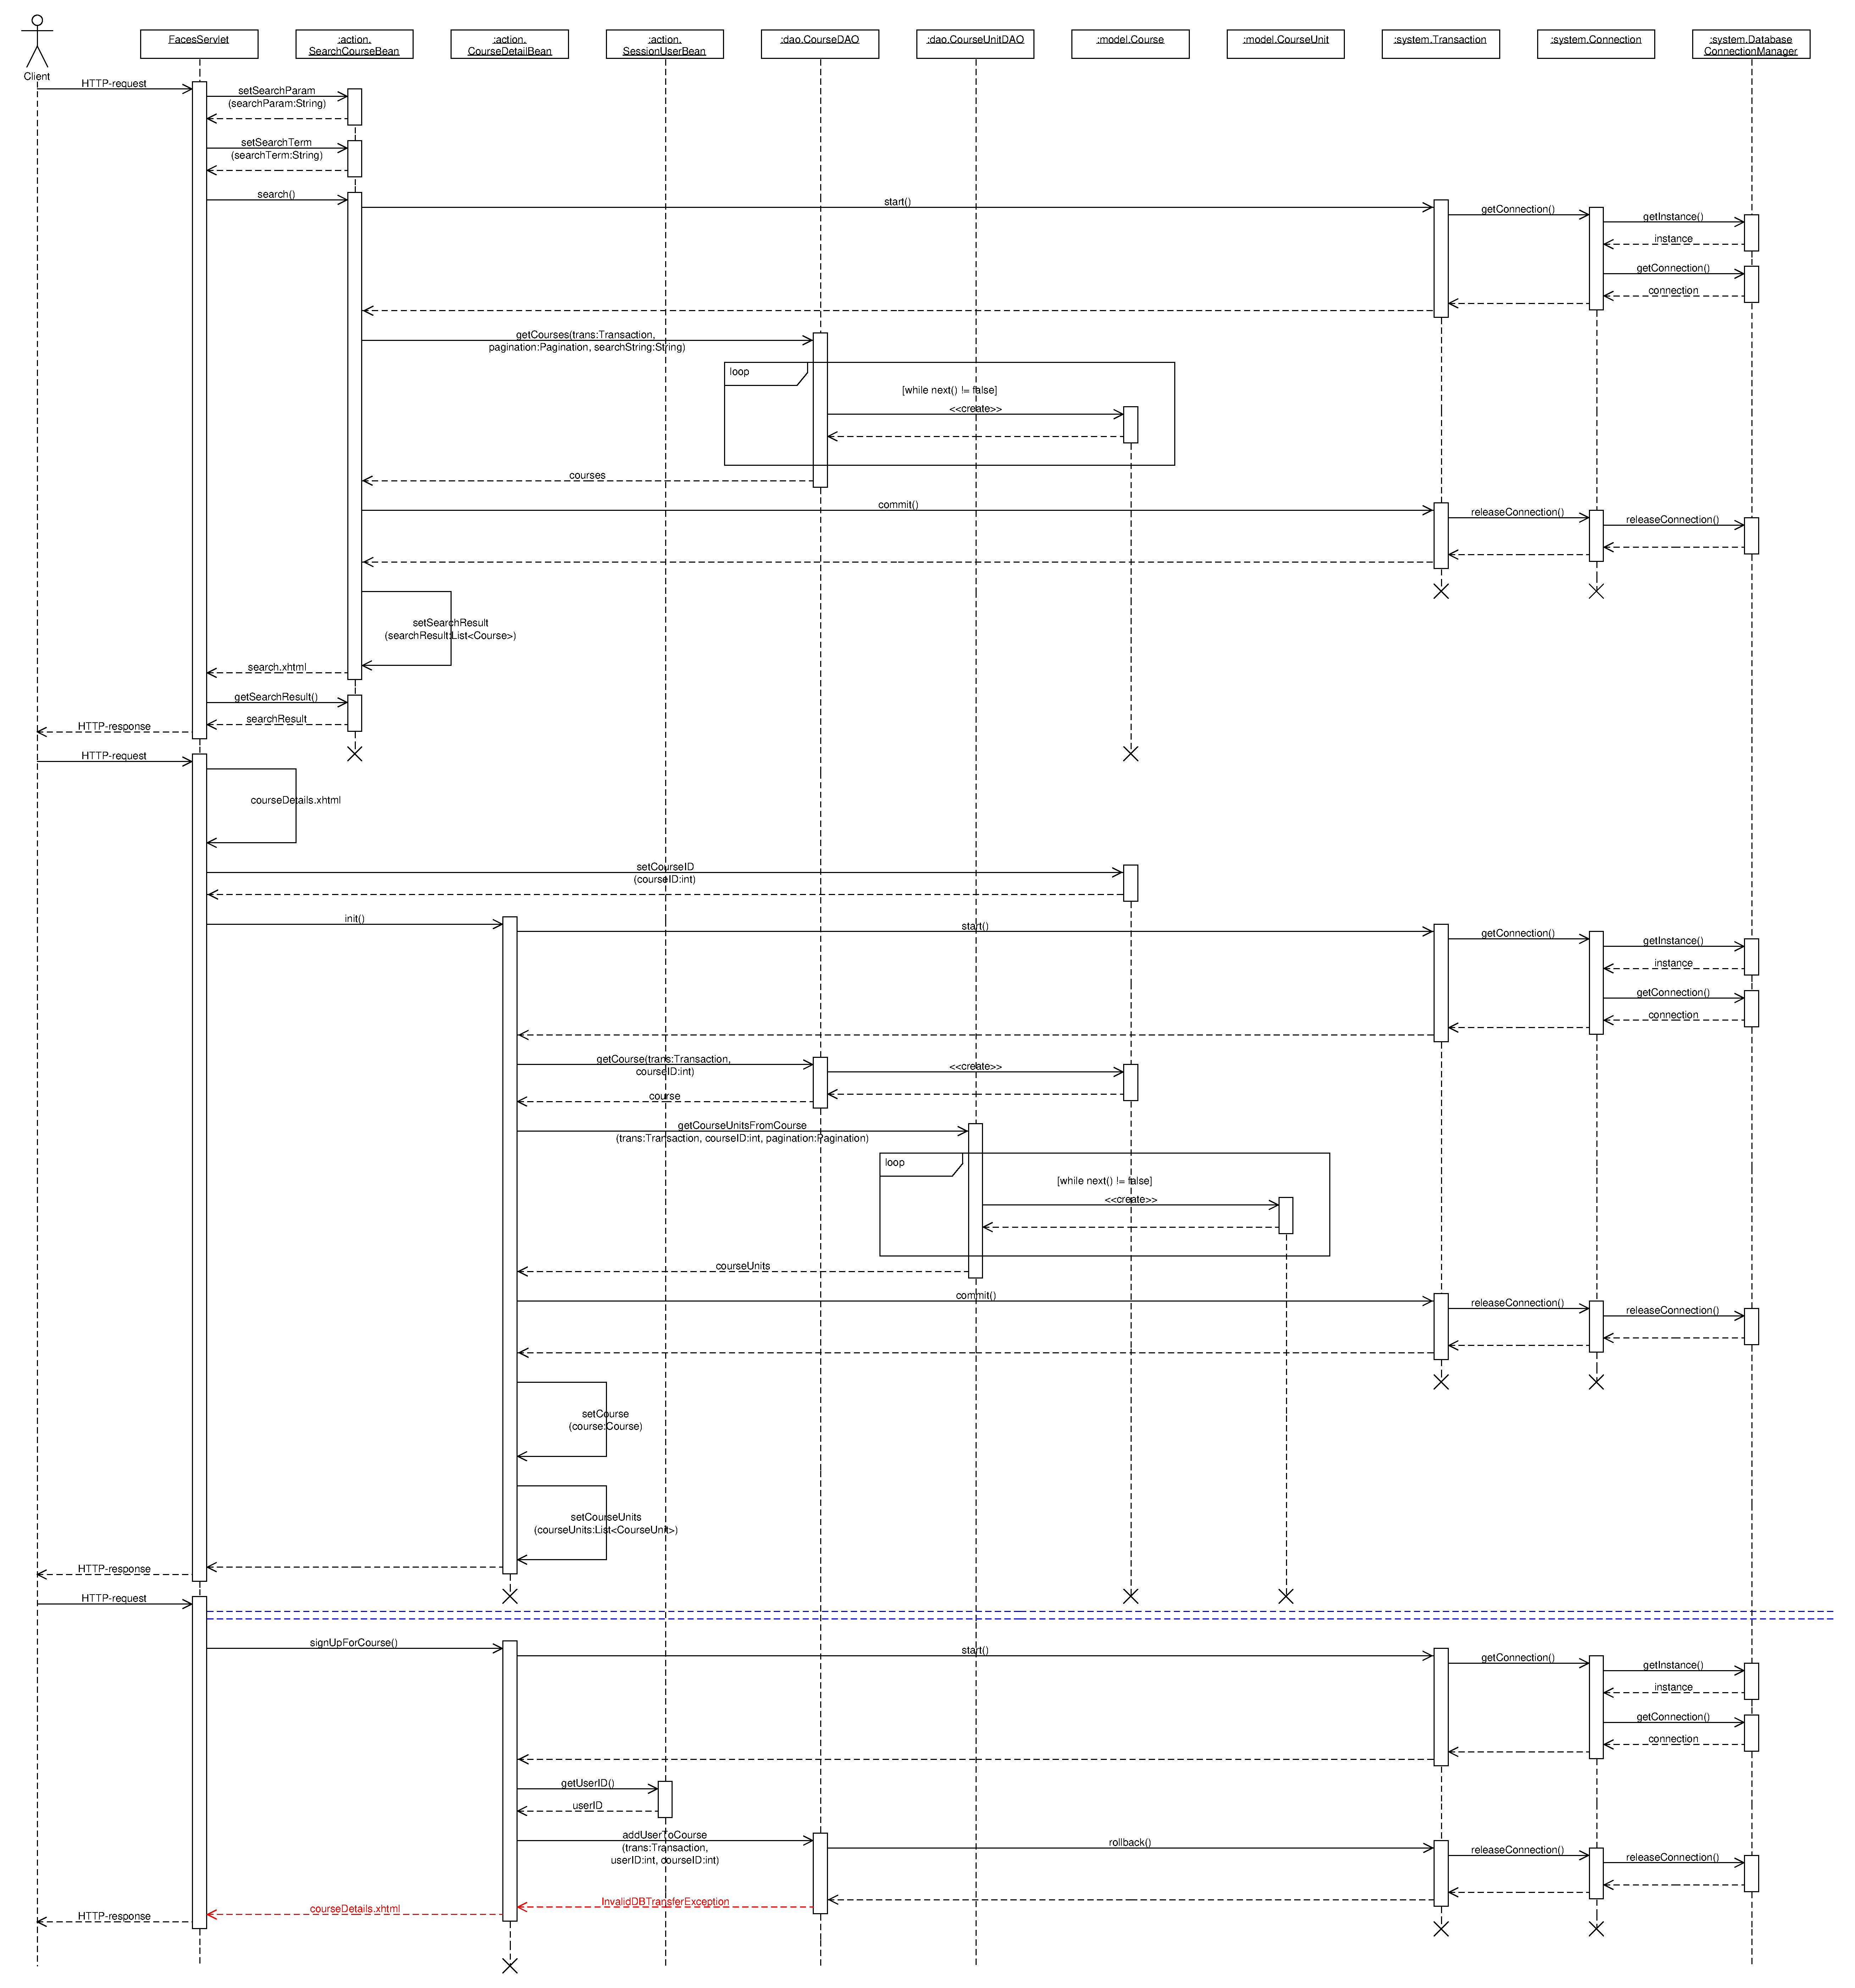
\includegraphics[scale=0.205]{./Grafiken/Sequenzdiagramm-Kursanmeldung.pdf}



